% Jenkins pipeline: every stage is a gate. Compile: tectonic -X compile pipeline.tex
\documentclass[tikz,border=4pt]{standalone}
\usepackage[T1]{fontenc}
\usepackage{tgheros}
\renewcommand*\familydefault{\sfdefault}
\usetikzlibrary{arrows.meta}
\definecolor{ink}{HTML}{0E0E0F}
\definecolor{muted}{HTML}{6B6965}
\definecolor{accent}{HTML}{C84A18}
\definecolor{soft}{HTML}{FDF0EA}
\begin{document}
\hyphenpenalty=10000\exhyphenpenalty=10000
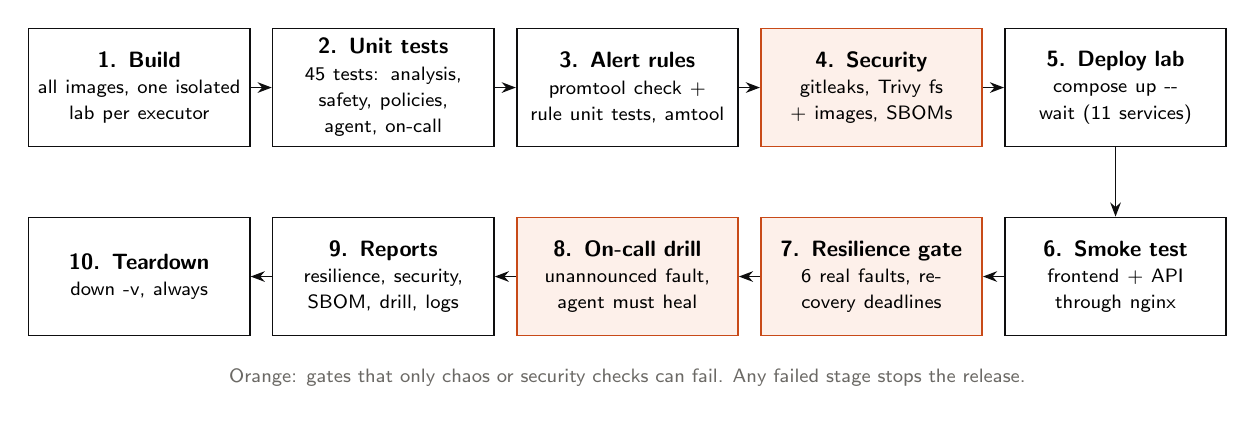
\begin{tikzpicture}[
  font=\footnotesize,
  st/.style={draw=ink, line width=0.6pt, fill=white, align=center, text width=26mm,
             minimum height=15mm, inner sep=3pt},
  gate/.style={st, draw=accent, fill=soft},
  arr/.style={-{Stealth[length=1.8mm]}, line width=0.6pt, draw=ink},
  note/.style={font=\scriptsize, text=muted, align=center},
]
\node[st] (s1) at (0,0) {{\bfseries 1. Build}\\ \scriptsize all images, one isolated lab per executor};
\node[st] (s2) at (3.1,0) {{\bfseries 2. Unit tests}\\ \scriptsize 45 tests: analysis, safety, policies, agent, on-call};
\node[st] (s3) at (6.2,0) {{\bfseries 3. Alert rules}\\ \scriptsize promtool check + rule unit tests, amtool};
\node[gate] (s4) at (9.3,0) {{\bfseries 4. Security}\\ \scriptsize gitleaks, Trivy fs + images, SBOMs};
\node[st] (s5) at (12.4,0) {{\bfseries 5. Deploy lab}\\ \scriptsize compose up {-}{-}wait (11 services)};
\node[st] (s6) at (12.4,-2.4) {{\bfseries 6. Smoke test}\\ \scriptsize frontend + API through nginx};
\node[gate] (s7) at (9.3,-2.4) {{\bfseries 7. Resilience gate}\\ \scriptsize 6 real faults, recovery deadlines};
\node[gate] (s8) at (6.2,-2.4) {{\bfseries 8. On-call drill}\\ \scriptsize unannounced fault, agent must heal};
\node[st] (s9) at (3.1,-2.4) {{\bfseries 9. Reports}\\ \scriptsize resilience, security, SBOM, drill, logs};
\node[st] (s10) at (0,-2.4) {{\bfseries 10. Teardown}\\ \scriptsize down -v, always};
\draw[arr] (s1) -- (s2); \draw[arr] (s2) -- (s3); \draw[arr] (s3) -- (s4); \draw[arr] (s4) -- (s5);
\draw[arr] (s5) -- (s6); \draw[arr] (s6) -- (s7); \draw[arr] (s7) -- (s8); \draw[arr] (s8) -- (s9);
\draw[arr] (s9) -- (s10);
\node[note, anchor=north] at (6.2,-3.45) {Orange: gates that only chaos or security checks can fail. Any failed stage stops the release.};
\end{tikzpicture}
\end{document}
